%%____________________________________________________________________________||
\section{Interpretation in Dark Matter models}
\label{sec:darkmatter}

In Run~1, the \alphat analysis searched for supersymmetry. Its results were used to interpret models with supersymmetry and their simplified
models. In Run~2, we extended the analysis strategy to include searches for the production of dark matter (DM) in the proton-proton collisions.

The properties of DM and their connections to known particles and
physical laws remain unknown. Although the Weakly Interacting Massive
Particles (WIMPs) hypothesis has guided the quest to understand this
fundamental problem, rapid experimental progress continues to exclude
large regions of the most popular dark matter models. In light of this
uncertainty, more model-independent searches for dark matter have gained
significant traction. It is important to be able to combine collider,
direct detection, and indirect detection searches in a complementary way
if we are to determine that a signal observed experimentally is indeed
from dark matter \cite{Bauer:2013ihz}.

In particular, the use of simplified models provides allows one to relate the different experimental
signatures in a relatively model-independent way~\cite{Buchmueller:2014yoa}. 

%Here it is assumed that new particles mediate the interactions between dark matter and standard model
%particles, but that these mediators are too heavy to be produced directly in experiments. Hence, the interactions can be described by a contact
%operator \cite{Beltran:2010ww}. For each operator and dark matter mass $m_\textrm{DM}$ the relic abundance, direct detection signal, and collider predictions depend on a single parameter $M_*$, which parameterizes the coupling strength of the contact interaction. 


The collider search for dark matter is a critical element of this
approach, and can provide the strongest constraints in cases where the
dark matter mass is $\lesssim 10\ \GeV$ or when the operator has
suppressed direct detection signals, e.g. in the case of
isospin-violating dark matter~\cite{Feng:2011vu} or pseudo-scalar
couplings~\cite{Buckley:2014fba}. The generic signature of dark matter
pair production in colliders is missing transverse momentum from the
dark matter and energetic visible particles that are used to tag the
event. First analyses using this final state used contact
operators~\cite{Goodman:2010ku} with couplings between dark matter and
quarks. The resulting ``monojet'' final state consisting of one or two
hard jets plus large missing transverse momentum from the dark matter.
Experimental limits using monojet final states have been published using
7 and 8 TeV LHC data \cite{Chatrchyan:2012me,ATLAS:2012ky} for a variety
of operators.
%In addition, similar final states with the form $\chi \bar \chi + X$, where $\chi$ is the dark matter particle
%and $X$ can be a photon, jet, or other particle, have been studied in the context of effective operators These additional particles are initial state radiation (ISR) 
%radiated off from the interacting partons. (e.g. \cite{Goodman:2010yf,Fox:2011pm,Petriello:2008pu,Fox:2011fx}).


%Previous CMS analyses performed the search for new physics in the monojet final state, as detailed in References~\cite{Aad:2011xw, ATLAS:2012ky} using up to $4.7\,\fbi$ 
%of data with proton-proton collision at a center-of-mass energy of $\sqrt{s}=7\,\tev$. A conference note~\cite{ATLAS-CONF-2012-147} using 8$\,\tev$ data has also been published, 
%based on half of the 2012 dataset. 


The present document also describes the planned analysis of WIMP pair production in association with light and heavy quarks using the upcoming 13~TeV data set corresponding. 
Hadronic final states of the form $\chi \bar \chi + X$, where $\chi$ is the dark matter particle and $X$ can be one or several jets have been studied in the context of effective operators. These jets are either directly produced due in the interaction between SM and DM or are initial state radiation (ISR)  radiated off from the interacting partons (e.g. \cite{Goodman:2010yf,Fox:2011pm,Petriello:2008pu,Fox:2011fx}). As detailed in Ref.~\cite{Lin:2013sca, Artoni:2013zba} particular the use of heavy quarks, namely $b$- and top quarks take advantage of quark-mass dependency of scalar couplings. The quark mass dependency comes from minimal flavor violation assumptions. Further advantages gained by the use of third generation quarks is to extend the analysis to larger jet multiplicities and therefore larger signal acceptance compared to the monojet analysis. Thus accessing a unique and orthogonal phase space. 


This analysis will also set strongest constraints for low mass dark matter, and the strongest collider constraints across a wide range of masses. We will also start to probe excesses observed in direct detection experiment at energies of about 10 GeV in the DAMA (2008), CoGent (2010/11), CREST-II (2012) and CDMS (2013) experiments but also by the Fermi-LAT (2013) satellite indicating a DM particle of about 50 GeV mass. We expect to place stringent constraints on this phase space in the near future with the $13$~TeV run.




\subsection{Simplified Models}


The primary simplified models for Dirac fermion DM studied and recommended by the DM Forum for early LHC Run-2 searches are
are comprised of spin-0 and spin-1 mediators using $s$-channel and $t$-channel models.


We consider the case of a DM particle $\chi$ of mass $m_{\chi}$ that is a Dirac fermion and where the production proceeds via the exchange
of a spin-1 mediator $\Phi$ of mass $m_{\Phi}$ in the $s$-channel. Two models with vector (V) and axial-vector (AV) couplings are considered. The coupling to the standard model
$g_{\textrm SM}$ is assumed to be universal for all quark families and $g_{\textrm DM}$ is the couplings to the dark matter particles. Assuming that not additional visible or invisible particles contribute to the decay we use the minimal width determined by the choice of $g_{\textrm SM}$ and $g_{\textrm DM}$.
We specifically assume that the vector mediator does not couple to leptons. If such a coupling were present, it would have a minor effect in increasing the mediator width, but it
would also bring in constraints from measurements of the Drell-Yan process that would unnecessarily restrict the model space. 
 In order to determine an optimal choice of the parameter grid for the simulation of early Run-2 benchmark models, dependencies of the kinematic quantities and cross sections on the model parameters
have been studied. Only points that are kinematically distinct will be fully simulated, while instructions on how to rescale the results
according to models with different cross sections. 


$M_{\Phi}$ grid points are chosen, roughly equidistant in a logarithmic scale: 10,~20, 50, 100, 200, 300, 500, 1000 and 2000 GeV. In the thresh-
old regime $M_{\Phi} = 2 \times m_{\Chi}$, the $ m_{\Chi}$ grid points are taken at approximately $M_{\Phi}/2$. Points on the on-shell diagonal are always chosen to be
5 GeV away from the threshold, to avoid numerical instabilities in the event generation. 


\begin{table}[h]
\centering
\begin{tabular}{l|llllllllll}\hline
mDM  & \multicolumn{10}{c}{mPhi}                                   \\ \hline
1    & 10 & 20 & 50 & 100 & 200 & 300 & 500 & 1000 & 2000 & 100000 \\
10   & 10 & 15 & 50 & 100 &     &     &     &      &      & 100000 \\
50   & 10 &    & 50 & 95  & 200 & 300 &     &      &      & 100000 \\
150  & 10 &    &    &     & 200 & 295 & 500 & 1000 &      & 100000 \\
500  & 10 &    &    &     &     &     & 500 & 995  &      & 100000 \\
1000 & 10 &    &    &     &     &     &     & 1000 & 1995 & 100000\\ \hline
\end{tabular}
\caption{Dark matter and mediator mass grid analysed. The parameter space follows the DM Forum recommendations}
\label{tab:DMgrid}
\end{table}

\subsubsection{Vector and Axial Vector Models}
\begin{table}[h]
\centering
\begin{tabular}{llllll}
\hline
sample             & $\sigma$ [pb] & Sum Evts       & Evts Sym. Bin & Evts Asym. Bin & Eff  [\%]   \\\hline
A\_mDM100\_mMed400  & 6.89E+01 & 4685.76 & 2271.72 & 2414.04 & 2.27 \\
A\_mDM10\_mMed1100  & 3.98E+00 & 192.57  & 91.15   & 101.42  & 1.61 \\
A\_mDM10\_mMed800   & 1.25E+01 & 811.34  & 399.56  & 411.78  & 2.17 \\
A\_mDM150\_mMed400  & 3.26E+01 & 1319.08 & 616.48  & 702.6   & 1.35 \\
A\_mDM200\_mMed1100 & 2.46E+00 & 243.48  & 113.89  & 129.59  & 3.3  \\
A\_mDM200\_mMed800  & 6.10E+00 & 544.81  & 252.92  & 291.89  & 2.98 \\
A\_mDM250\_mMed400  & 3.07E+00 & 168.19  & 78.77   & 89.42   & 1.82 \\
A\_mDM300\_mMed1100 & 1.57E+00 & 93.84   & 45.12   & 48.71   & 1.99 \\
A\_mDM300\_mMed800  & 2.72E+00 & 207.65  & 100.6   & 107.05  & 2.55 \\
A\_mDM350\_mMed400  & 6.01E-01 & 41.03   & 19.01   & 22.02   & 2.28 \\
A\_mDM400\_mMed1100 & 8.33E-01 & 86.83   & 43.47   & 43.36   & 3.47 \\
A\_mDM400\_mMed800  & 8.08E-01 & 97.91   & 46.89   & 51.02   & 4.04 \\
A\_mDM450\_mMed400  & 1.86E-01 & 21.81   & 10.97   & 10.84   & 3.91 \\
A\_mDM500\_mMed1100 & 3.41E-01 & 49.13   & 22.9    & 26.23   & 4.8  \\
A\_mDM500\_mMed800  & 2.04E-01 & 17.94   & 8.44    & 9.5     & 2.93 \\
A\_mDM50\_mMed400   & 1.06E+02 & 2660.98 & 1194.5  & 1466.48 & 0.84\\
\hline
\hline
\end{tabular}
\caption{Selected axial-vector samples. Given are production cross section, event yields for 3 $fb^{-1 }$ for the various selections and the overall selection efficiency for $g_DM=g_SM=1$}
\label{tab:dm_A_g1_3fb}
\end{table}


\begin{table}[h]
\centering
\begin{tabular}{llllll}
\hline
sample             & $\sigma$ [pb] & Sum Evts       & Evts Sym. Bin & Evts Asym. Bin & Eff  [\%]   \\\hline
V\_mDM100\_mMed400  & 9.49E+01 & 3038.09 & 1445.03 & 1593.07 & 1.07 \\
V\_mDM10\_mMed1100  & 3.89E+00 & 360.59  & 177.59  & 182.99  & 3.09 \\
V\_mDM10\_mMed800   & 1.19E+01 & 692.38  & 317.41  & 374.97  & 1.94 \\
V\_mDM150\_mMed400  & 6.98E+01 & 1943.39 & 923.21  & 1020.18 & 0.93 \\
V\_mDM200\_mMed1100 & 3.28E+00 & 244.74  & 116.17  & 128.58  & 2.49 \\
V\_mDM200\_mMed800  & 9.37E+00 & 745.95  & 346.92  & 399.03  & 2.65 \\
V\_mDM250\_mMed400  & 1.08E+01 & 902.86  & 447.89  & 454.97  & 2.79 \\
V\_mDM300\_mMed1100 & 2.73E+00 & 341.49  & 174.71  & 166.79  & 4.17 \\
V\_mDM300\_mMed800  & 6.50E+00 & 392.12  & 184.01  & 208.11  & 2.01 \\
V\_mDM350\_mMed400  & 1.99E+00 & 100.42  & 47.38   & 53.05   & 1.68 \\
V\_mDM400\_mMed1100 & 2.02E+00 & 107.53  & 52.22   & 55.31   & 1.77 \\
V\_mDM400\_mMed800  & 3.02E+00 & 242.18  & 117.44  & 124.74  & 2.67 \\
V\_mDM450\_mMed400  & 6.24E-01 & 45.69   & 21.84   & 23.85   & 2.44 \\
V\_mDM500\_mMed1100 & 1.18E+00 & 79.23   & 38.63   & 40.6    & 2.24 \\
V\_mDM500\_mMed800  & 8.22E-01 & 70.33   & 33.94   & 36.39   & 2.85 \\
V\_mDM50\_mMed400   & 1.08E+02 & 3248.04 & 1511.08 & 1736.96 & 1.00 \\
\hline
\end{tabular}
\caption{Selected vector samples. Given are production cross section, event yields for 3 $fb^{-1 }$ for the various selections and the overall selection efficiency for $g_DM=g_SM=1$}
\label{tab:dm_V_g1_3fb}
\end{table}

\subsubsection{Scalar and Pseudoscalar Models} \label{sec:dm_pscalar}

\begin{table}[h]
\centering
\begin{tabular}{llllll}
\hline
sample             & $\sigma$ [pb] & Sum Evts       & Evts Sym. Bin & Evts Asym. Bin & Eff  [\%]   \\\hline
S\_mDM100\_mMed350 & 2.31E+00 & 126.62 & 53.47  & 73.15  & 1.82 \\
S\_mDM10\_mMed225  & 5.71E+00 & 266.19 & 95.96  & 170.22 & 1.55 \\
S\_mDM10\_mMed50   & 2.66E+01 & 295.33 & 114.41 & 180.93 & 0.37 \\
S\_mDM125\_mMed400 & 1.59E+00 & 89.97  & 39.81  & 50.16  & 1.88 \\
S\_mDM150\_mMed400 & 9.79E-01 & 59.63  & 24.09  & 35.54  & 2.03 \\
S\_mDM15\_mMed250  & 4.94E+00 & 239.01 & 106.17 & 132.84 & 1.61 \\
S\_mDM15\_mMed75   & 1.84E+01 & 337.76 & 122.99 & 214.77 & 0.61 \\
S\_mDM1\_mMed25    & 5.02E+01 & 430.66 & 186.79 & 243.87 & 0.29 \\
S\_mDM200\_mMed275 & 1.23E-02 & 1.06   & 0.49   & 0.57   & 2.86 \\
S\_mDM20\_mMed150  & 9.07E+00 & 275.78 & 116.12 & 159.66 & 1.01 \\
S\_mDM20\_mMed400  & 3.30E+00 & 203.51 & 90.19  & 113.32 & 2.05 \\
S\_mDM35\_mMed225  & 4.96E+00 & 218.64 & 94.7   & 123.95 & 1.47 \\
S\_mDM35\_mMed50   & 3.44E-01 & 11.95  & 5.37   & 6.58   & 1.16 \\
S\_mDM50\_mMed275  & 3.66E+00 & 192.7  & 81.17  & 111.52 & 1.76 \\
S\_mDM5\_mMed10    & 3.81E+00 & 46.88  & 19.82  & 27.06  & 0.41 \\
S\_mDM5\_mMed300   & 4.18E+00 & 221.37 & 94.39  & 126.97 & 1.77 \\
S\_mDM75\_mMed150  & 3.18E-01 & 13.47  & 5.21   & 8.26   & 1.41 \\
S\_mDM75\_mMed450  & 1.82E+00 & 120.5  & 56.16  & 64.34  & 2.21\\
\hline
\end{tabular}
\caption{Selected scalar samples. Given are production cross section, event yields for 3 $fb^{-1 }$ for the various selections and the overall selection efficiency for $g_DM=g_SM=1$}
\label{tab:dm_S_g1_3fb}
\end{table}


\begin{table}[h]
\centering
\begin{tabular}{llllll}
\hline
sample             & $\sigma$ [pb] & Sum Evts       & Evts Sym. Bin & Evts Asym. Bin & Eff  [\%]   \\\hline
P\_mDM100\_mMed350 & 1.25E+01 & 632.71  & 265.81  & 366.9   & 1.69 \\
P\_mDM10\_mMed200  & 1.66E+01 & 668.92  & 282.88  & 386.04  & 1.34 \\
P\_mDM10\_mMed500  & 2.10E+00 & 165.24  & 70.13   & 95.12   & 2.62 \\
P\_mDM125\_mMed350 & 1.06E+01 & 574.48  & 230.85  & 343.62  & 1.8  \\
P\_mDM150\_mMed350 & 7.83E+00 & 389.76  & 154.97  & 234.8   & 1.66 \\
P\_mDM15\_mMed250  & 1.33E+01 & 631.37  & 262.63  & 368.74  & 1.59 \\
P\_mDM15\_mMed75   & 4.97E+01 & 809.62  & 302.99  & 506.63  & 0.54 \\
P\_mDM1\_mMed25    & 1.14E+02 & 1013.45 & 375.77  & 637.68  & 0.3  \\
P\_mDM200\_mMed275 & 7.09E-02 & 5.52    & 2.42    & 3.1     & 2.6  \\
P\_mDM20\_mMed150  & 2.30E+01 & 709.86  & 281.18  & 428.68  & 1.03 \\
P\_mDM20\_mMed400  & 6.73E+00 & 389.39  & 158.04  & 231.34  & 1.93 \\
P\_mDM35\_mMed225  & 1.40E+01 & 601.6   & 249.85  & 351.75  & 1.44 \\
P\_mDM35\_mMed50   & 1.41E+00 & 38.92   & 14.67   & 24.26   & 0.92 \\
P\_mDM50\_mMed275  & 1.18E+01 & 564.9   & 220.54  & 344.37  & 1.6  \\
P\_mDM5\_mMed10    & 8.66E+02 & 5888.89 & 3117.65 & 2771.24 & 0.23 \\
P\_mDM5\_mMed300   & 1.27E+01 & 657.28  & 263.93  & 393.35  & 1.73 \\
P\_mDM75\_mMed150  & 9.49E+01 & 3199.78 & 1300.8  & 1898.98 & 1.12 \\
P\_mDM75\_mMed450  & 3.39E+00 & 237.3   & 106.45  & 130.86  & 2.33 \\
\hline
\end{tabular}
\caption{Selected pseudo-scalar samples. Given are production cross section, event yields for 3 $fb^{-1 }$ for the various selections and the overall selection efficiency for $g_DM=g_SM=1$}
\label{tab:dm_P_g1_3fb}
\end{table}


\subsubsection{Heavy Quark Models}

Following the concept of Minimal Flavor Violating (MFV) top and bottom quarks can play important roles in the phenomenology of dark matter events.
Scalar and pseudoscalar mediator models predict not only the monojet process described in Sec.~\ref{sec:dm_pscalar} but also production of dark matter in association
with top (or bottom) pairs. This results in signature with relative large jet multiplicities, in particular for DM$+t\bar{t}$ production and heavy jets. Our $\alpa_{\textrm{T}}$ is particular well designed for this signature and the aforementioned improvements for monojet-like and compressed events further improves the sensitivity. The events are produced in the same parameters space as detailed in Tab.~\ref{tab:DMgrid} using \textsc{MadGraph5\_aMC@NLO} 2.2.2 and using \textsc{Pythia 8} for the parton shower.



\begin{table}[h]
\centering
\begin{tabular}{l|lllll}
\hline
sample             & $\sigma$ [pb] & Sum Evts       & Evts Sym. Bin & Evts Asym. Bin & Eff  [\%]   \\\hline
Mchi1000\_MPhi10\_g1  & 6.60E-09 & 0.00   & 0.00   & 0.00  & 29.94 \\
Mchi100\_MPhi100\_g1  & 3.24E-04 & 0.20   & 0.16   & 0.04  & 20.27 \\
Mchi100\_MPhi300\_g1  & 2.91E-02 & 17.14  & 13.61  & 3.53  & 19.66 \\
Mchi10\_MPhi10\_g1    & 9.47E-02 & 13.08  & 11.12  & 1.96  & 4.61  \\
Mchi10\_MPhi250\_g1   & 4.84E-02 & 25.67  & 20.25  & 5.42  & 17.69 \\
Mchi150\_MPhi10\_g1   & 8.66E-05 & 0.06   & 0.05   & 0.01  & 21.95 \\
Mchi150\_MPhi5000\_g1 & 4.17E-08 & 0.00   & 0.00   & 0.00  & 26.07 \\
Mchi1\_MPhi100\_g1    & 6.72E-01 & 158.06 & 128.24 & 29.82 & 7.85  \\
Mchi1\_MPhi200\_g1    & 9.34E-02 & 40.74  & 31.78  & 8.95  & 14.54 \\
Mchi1\_MPhi5000\_g1   & 6.15E-08 & 0.00   & 0.00   & 0.00  & 23.47 \\
Mchi500\_MPhi10\_g1   & 7.39E-07 & 0.00   & 0.00   & 0.00  & 27.15 \\
Mchi500\_MPhi500\_g1  & 9.93E-07 & 0.00   & 0.00   & 0.00  & 26.77 \\
Mchi50\_MPhi200\_g1   & 9.23E-02 & 40.63  & 31.54  & 9.09  & 14.67 \\
Mchi50\_MPhi50\_g1    & 2.33E-03 & 0.92   & 0.74   & 0.18  & 13.19 \\
\hline
\end{tabular}
\caption{Selected DM+$t\bar{t}$ scalar samples. Given are production cross section, event yields for 3 $fb^{-1 }$ for the various selections and the overall selection efficiency for $g_DM=g_SM=1$}
\label{tab:dm_dmtt_S_g1}
\end{tabular}
\end{table}

\begin{table}[h]
\centering
\begin{tabular}{l|lllll}
\hline
sample             & $\sigma$ [pb] & Sum Evts       & Evts Sym. Bin & Evts Asym. Bin & Eff  [\%]   \\\hline
Mchi1000\_MPhi10\_g1  & 2.59E-08 & 0.00   & 0.00  & 0.00  & 29.83 \\
Mchi100\_MPhi1000\_g1 & 3.84E-04 & 0.29   & 0.24  & 0.05  & 25.11 \\
Mchi100\_MPhi195\_g1  & 5.93E-03 & 3.11   & 2.39  & 0.72  & 17.45 \\
Mchi10\_MPhi100\_g1   & 1.90E-01 & 77.50  & 59.95 & 17.55 & 13.58 \\
Mchi10\_MPhi200\_g1   & 8.40E-02 & 41.68  & 32.05 & 9.63  & 16.53 \\
Mchi10\_MPhi50\_g1    & 3.01E-01 & 102.82 & 78.50 & 24.31 & 11.38 \\
Mchi150\_MPhi295\_g1  & 3.38E-03 & 1.91   & 1.47  & 0.44  & 18.87 \\
Mchi1\_MPhi1000\_g1   & 3.97E-04 & 0.30   & 0.24  & 0.05  & 24.82 \\
Mchi1\_MPhi2000\_g1   & 1.09E-05 & 0.01   & 0.01  & 0.00  & 26.93 \\
Mchi1\_MPhi300\_g1    & 4.01E-02 & 22.73  & 17.57 & 5.16  & 18.91 \\
Mchi50\_MPhi50\_g1    & 2.97E-03 & 1.48   & 1.13  & 0.34  & 16.59
\hline
\end{tabular}
\caption{Selected DM+$t\bar{t}$ pseudo-scalar samples. Given are production cross section, event yields for 3 $fb^{-1 }$ for the various selections and the overall selection efficiency for $g_DM=g_SM=1$}
\label{tab:dm_dmtt_P_g1}
\end{tabular}
\end{table}



\subsection{EFT samples}
Table~\ref{tab:datasets_dm} lists the EFT samples generated using full simulation for the Phys14 exercise. The samples are generated using a mediator mass $M=40$~TeV.
\begin{sidewaystable}[h]
    \centering
    \caption{EFT dark matter samples for axial-vector and axial couplings using a mediator mass $M=40$~TeV \label{tab:datasets_dm}}
    \begin{tabular}{lr}
      \hline\hline
      \multicolumn{1}{c}{Data set}&\multicolumn{1}{c}{\# events}\tabularnewline
      \hline
      {\footnotesize \verb!/DarkMatter_Monojet_M-1_V_Tune4C_13TeV-madgraph/Phys14DR-PU20bx25_PHYS14_25_V1-v1/MINIAODSIM!   } &$197200$\tabularnewline
      {\footnotesize \verb!/DarkMatter_Monojet_M-100_V_Tune4C_13TeV-madgraph/Phys14DR-PU20bx25_PHYS14_25_V1-v1/MINIAODSIM! } &$189400$\tabularnewline
      {\footnotesize \verb!/DarkMatter_Monojet_M-1000_V_Tune4C_13TeV-madgraph/Phys14DR-PU20bx25_PHYS14_25_V1-v1/MINIAODSIM!} &$197200$\tabularnewline
      {\footnotesize \verb!/DarkMatter_Monojet_M-10_V_Tune4C_13TeV-madgraph/Phys14DR-PU20bx25_PHYS14_25_V1-v1/MINIAODSIM!  } &$191800$\tabularnewline
      {\footnotesize \verb!/DarkMatter_Monojet_M-1_AV_Tune4C_13TeV-madgraph/Phys14DR-PU20bx25_PHYS14_25_V1-v1/MINIAODSIM!  } &$191200$\tabularnewline
      {\footnotesize \verb!/DarkMatter_Monojet_M-10_AV_Tune4C_13TeV-madgraph/Phys14DR-PU20bx25_PHYS14_25_V1-v1/MINIAODSIM! } &$191200$\tabularnewline
      {\footnotesize \verb!/DarkMatter_Monojet_M-100_AV_Tune4C_13TeV-madgraph/Phys14DR-PU20bx25_PHYS14_25_V1-v1/MINIAODSIM!} &$191200$\tabularnewline
\hline
\end{tabular}
\end{sidewaystable}


\subsubsection{Light Jet EFT}

\begin{table}[h]
\centering
\begin{tabular}{llllll}
\hline
sample             & $\sigma$ [pb] & Sum Evts       & Evts Sym. Bin & Evts Asym. Bin & Eff  [\%]   \\\hline
\multicolumn{6}{c}{axial-vector}        \\\line
1    & 9.57E-01 & 554.17 & 329.48 & 224.68 & 19.3  \\
10   & 9.54E-01 & 554.94 & 332.06 & 222.88 & 19.39 \\
100  & 8.01E-01 & 507.55 & 305.86 & 201.68 & 21.12 \\
1000 & 4.66E-02 & 39.05  & 24.21  & 14.84  & 27.91 \\
\multicolumn{6}{c}{vector}        \\\line
110    & 9.55E-01 & 553.96 & 331.02 & 222.94 & 19.34 \\
100   & 9.05E-01 & 544.63 & 323.4  & 221.22 & 20.07 \\
1000  & 1.24E-01 & 102.45 & 63.73  & 38.72  & 27.46 \\
\hline
\end{tabular}
\caption{Yields for the light jet EFT sampels for $3\fbinv$.} 
\label{tab:dm_mj_eft_yields}
\end{table}


\begin{table}[h]
\centering
\begin{tabular}{lll}\hline
$m_{\textrm{DM}}$& $3\fbinv$  & $10\fbinv$ \\\hline
5\multicolumn{3}{c}{axial-vector}        \\\line
1             & 0.41 & 0.24 \\
10            & 0.40 & 0.23 \\
100           & 0.42 & 0.25 \\
1000          & 4.02 & 2.26 \\\hline
\multicolumn{3}{c}{vector}        \\\line
10            & 0.41 & 0.24 \\
100           & 0.40 & 0.24 \\
1000          & 1.55 & 0.87\\
\hline
\end{tabular}
\caption{Expected R values for the (axial)-vector EFT model for $3\fbinv$ and $10\fbinv$.} 
\label{tab:dm_mj_eft_rvalues}
\end{table}


\begin{figure}[h]
  \centering
  \subfigure{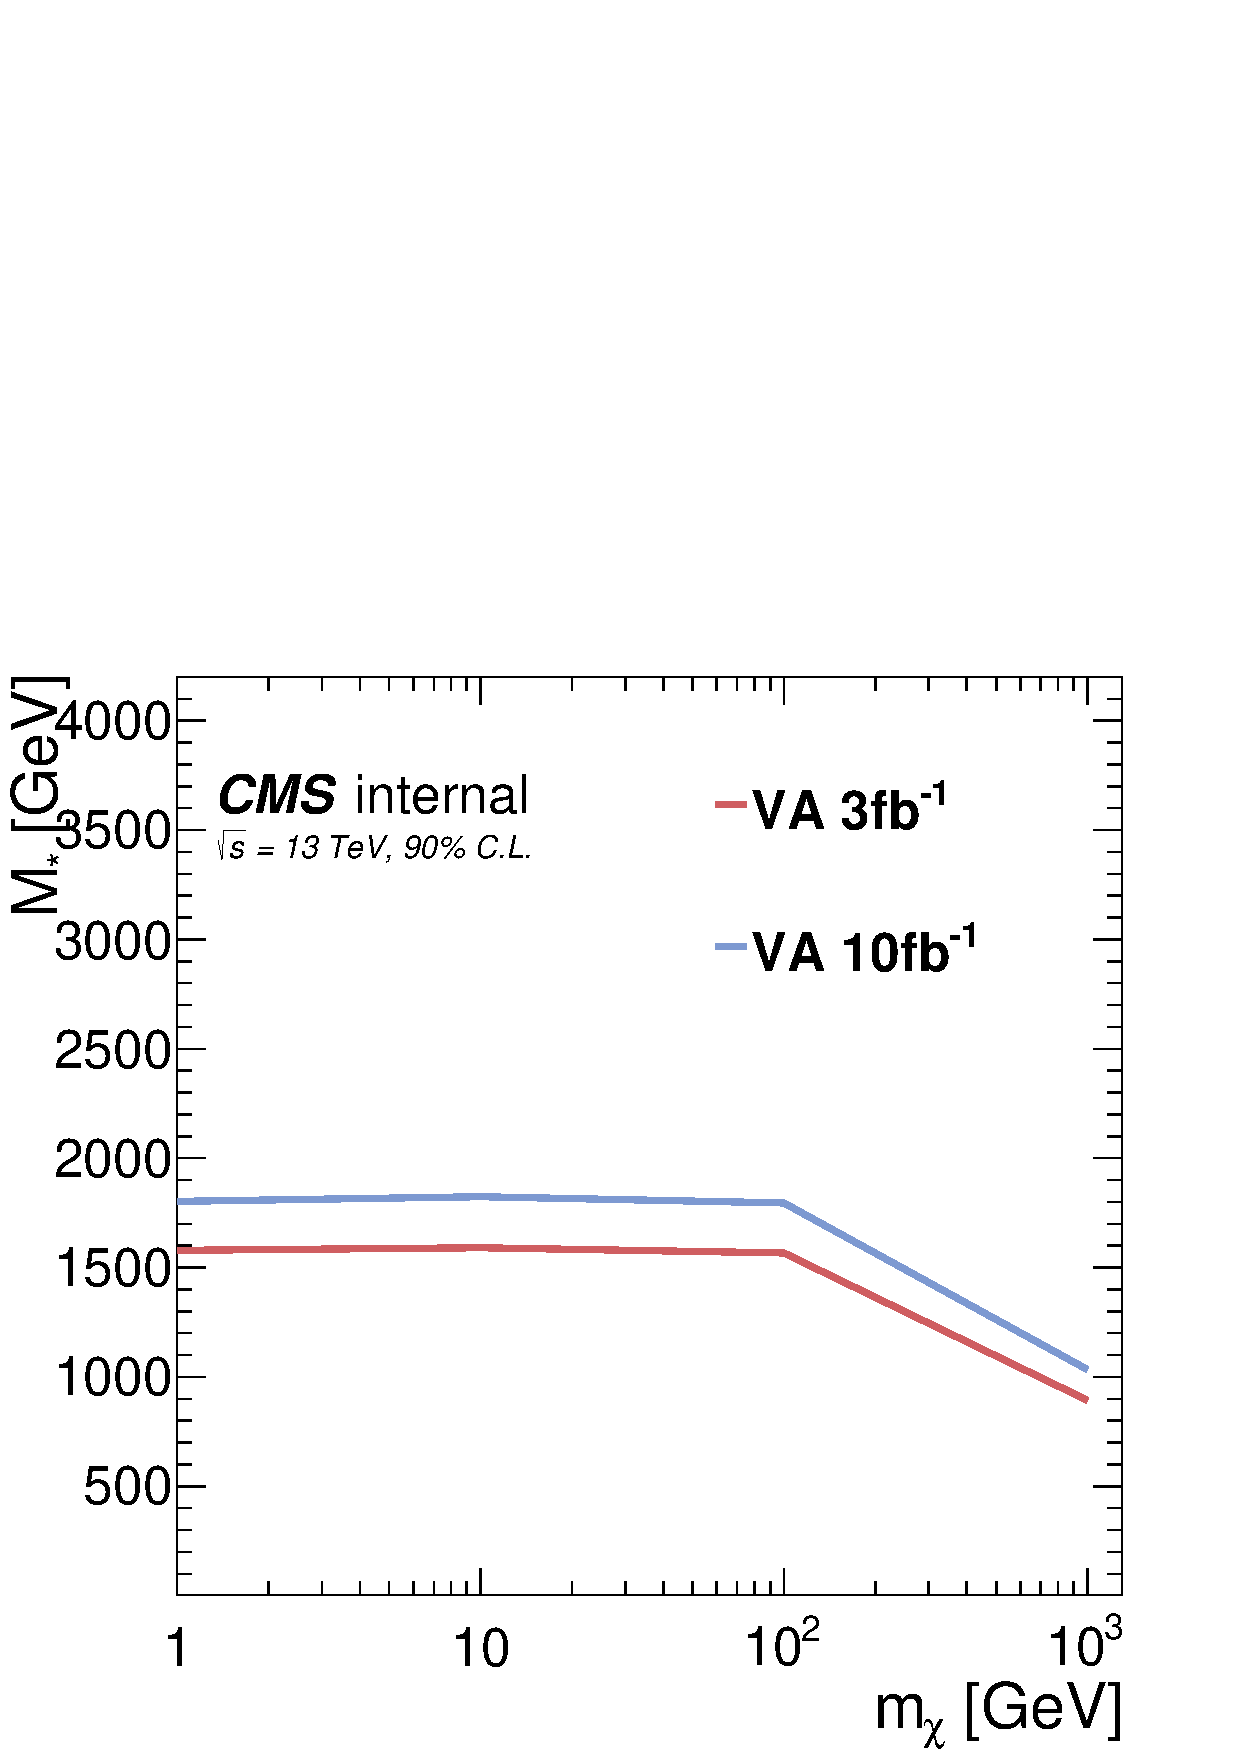
\includegraphics[width=0.7\textwidth]{figures/DMplots/limit_EFT_MJ_90.pdf}}
  \caption{\label{fig:MJ_EFT_limit} Expected limits on $M^*$at 90\% CL for $3\fbinv$ and $10\fbinv$ using the light jet axial-vector EFT models. }
\end{figure}



\subsubsection{DM+tt EFT}

\begin{sidewaystable}[h]
    \centering
    \caption{EFT dark matter samples for scalar $DM+t\bar{t}$ samples using a mediator mass $M=1x$~TeV. The cross sections are scaled by $10^6$ which corresponds to $M_*=100$ GeV \label{tab:datasets_dm}}
    \begin{tabular}{lr}
      \hline\hline
      \multicolumn{1}{c}{Data set}&\multicolumn{1}{c}{\# events}\tabularnewline
      \hline
      {\footnotesize \verb!/TTDMDMJets_M1GeV_Tune4C_13TeV-madgraph-tauola/Phys14DR- PU20bx25_PHYS14_25_V1-v1/MINIAODSIM!}   & 1.32 \tabularnewline
      {\footnotesize \verb!/TTDMDMJets_M10GeV_Tune4C_13TeV-madgraph-tauola/Phys14DR- PU20bx25_PHYS14_25_V1-v1/MINIAODSIM!}  & 1.32 \tabularnewline
      {\footnotesize \verb!/TTDMDMJets_M50GeV_Tune4C_13TeV-madgraph-tauola/Phys14DR- PU20bx25_PHYS14_25_V1-v1/MINIAODSIM!}  & 1.19 \tabularnewline
      {\footnotesize \verb!/TTDMDMJets_M200GeV_Tune4C_13TeV-madgraph-tauola/Phys14DR- PU20bx25_PHYS14_25_V1-v1/MINIAODSIM!} & 0.63 \tabularnewline
      {\footnotesize \verb!/TTDMDMJets_M600GeV_Tune4C_13TeV-madgraph-tauola/Phys14DR- PU20bx25_PHYS14_25_V1-v1/MINIAODSIM!} & 0.10 \tabularnewline
      {\footnotesize \verb!/TTDMDMJets_M1000GeV_Tune4C_13TeV-madgraph-tauola/Phys14DR- PU20bx25_PHYS14_25_V1-v1/MINIAODSIM!}& 0.02 \tabularnewline
      \hline \hline
\end{tabular}
\end{sidewaystable}

\begin{table}[h]
\centering
\begin{tabular}{llllll}
\hline
sample             & $\sigma$ [pb] & Sum Evts       & Evts Sym. Bin & Evts Asym. Bin & Eff  [\%]   \\\hline
1    & 1.32E+00 & 645.69 & 470.29 & 175.4  & 16.31 \\
10   & 1.32E+00 & 650.53 & 476.32 & 174.21 & 16.4  \\
50   & 1.19E+00 & 636.05 & 463.57 & 172.48 & 17.86 \\
200  & 6.30E-01 & 375.29 & 282.03 & 93.26  & 19.85 \\
600  & 1.04E-01 & 69.36  & 55.21  & 14.15  & 22.27\\
1000 & 1.58E-02 & 11.1   & 9.15   & 1.95   & 23.34 \\
\hline
\end{tabular}
\caption{Production cross section, event yields scaled to 3 $fb^{-1 }$ for the various selections and the overall selection efficiency for DM+$t\bar{t}$ EFT samples}
\label{tab:dm_dmtt_EFT_g1}
\end{table}


\begin{table}[h]
\centering
\begin{tabular}{lll}\hline
$m_{\textrm{DM}}$& $3\fbinv$  & $10\fbinv$ \\\hline
1            & 0.13 & 0.07 \\
10           & 0.09 & 0.05 \\
50           & 0.09 & 0.05 \\
200          & 0.13 & 0.07 \\
600          & 0.53 & 0.28 \\
1000         & 2.63 & 1.36 \\
\hline
\end{tabular}
\caption{Expected R values for the DM+$t\bar{t}$ EFT model for $3\fbinv$ and $10\fbinv$.} 
\label{tab:dm_dmtt_eft_rvalues}
\end{table}


\begin{figure}[h]
  \centering
  \subfigure{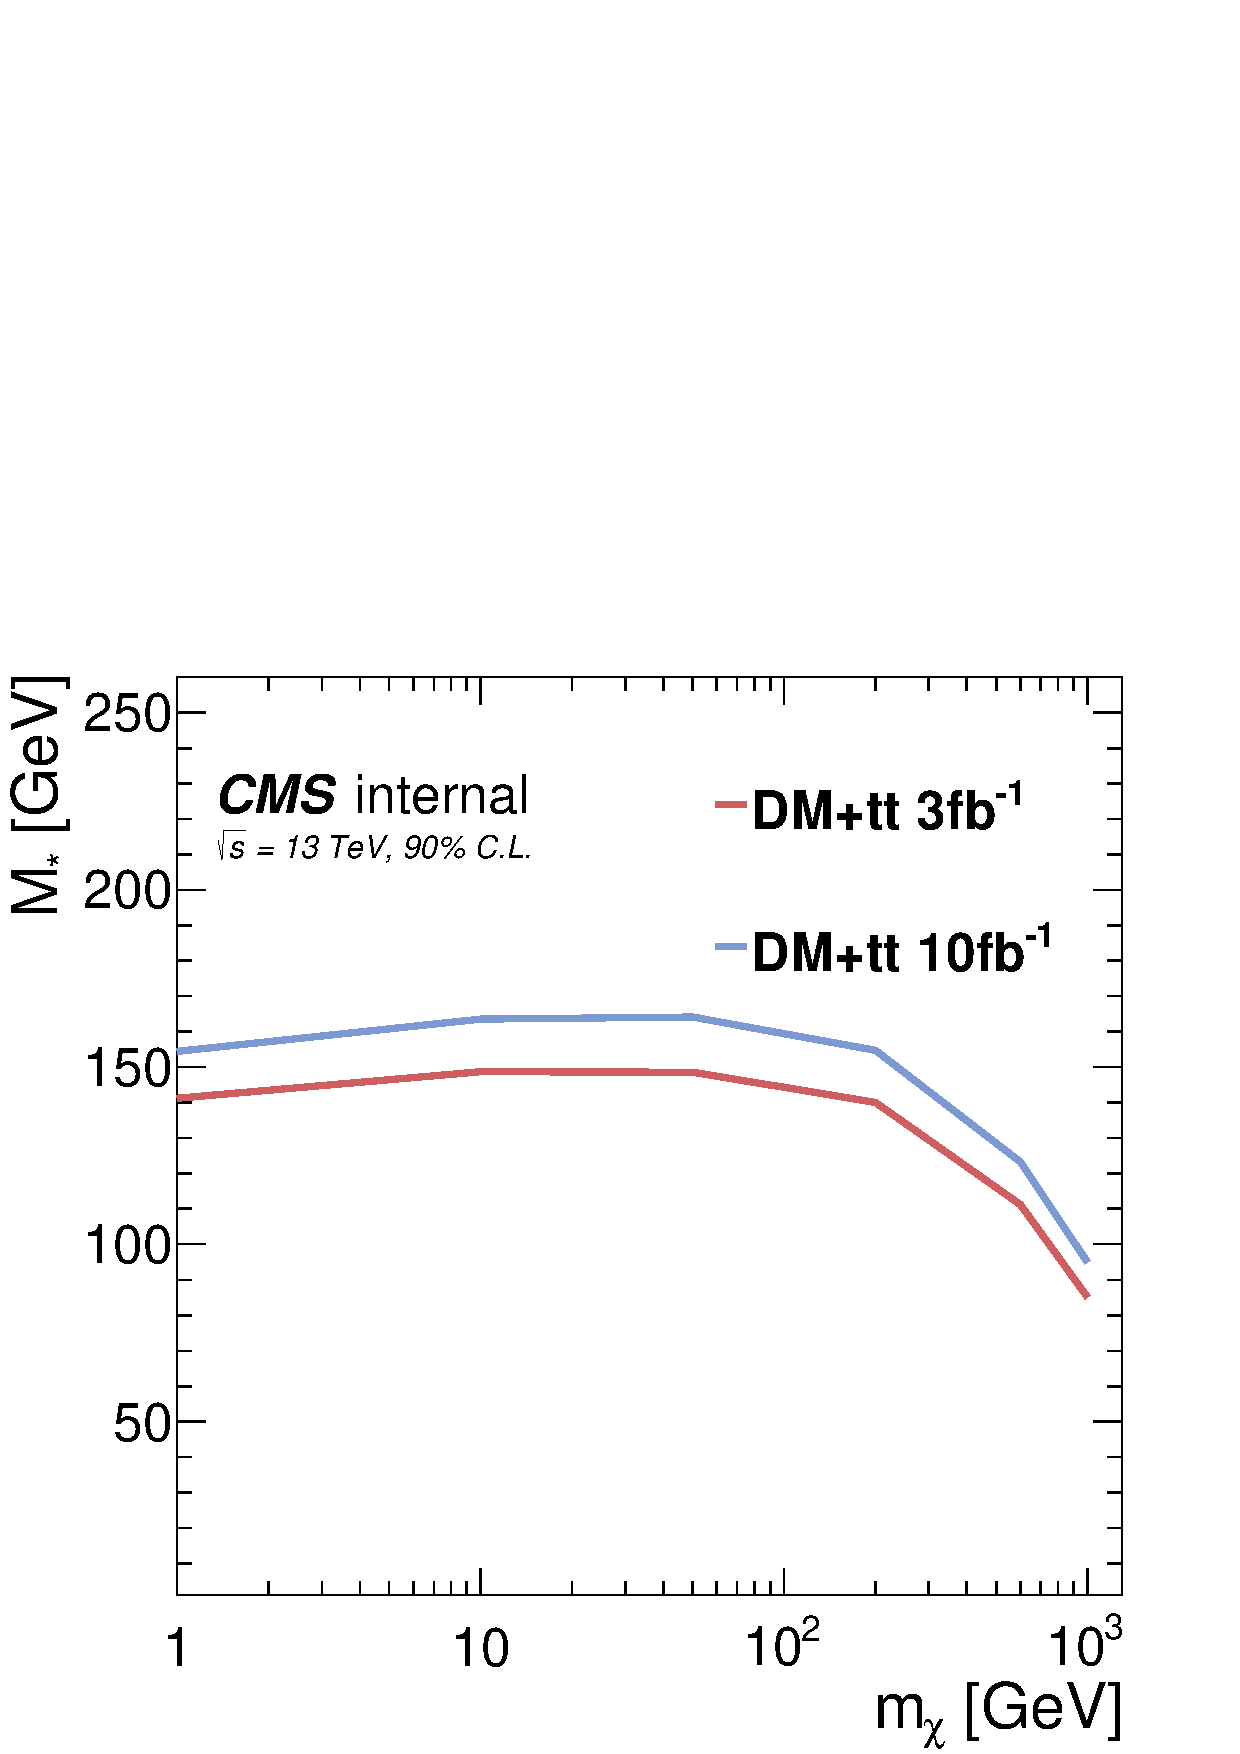
\includegraphics[width=0.7\textwidth]{figures/DMplots/limit_DMtt_EFT_90.pdf}}
  \caption{\label{fig:DMtt_EFT_limit} Expected limits on $M^*$at 90\% CL for $3\fbinv$ and $10\fbinv$ using a scalar DM+$t\bar{t}$ EFT model. }
\end{figure}


%%____________________________________________________________________________||
